The top production cross-section is substantially higher than the 
$\WW$ cross-section.
Thus the background due to top quarks represents a significant 
challenge for studies of the $\WW$ final state, including $H \to \WW$ searches. 

As explained in Section~\ref{sec:sel_toptag}, we use a dedicated top tagging 
veto, which relies on identifying $b$-quarks from top decay to 
further suppress the top background. 
By assessing the tagging efficiency and applying this to the number of
tagged events, we can estimate the residual top background after the veto.
Because details of the jet fragmentation cannot be reliably simulated at 
low energy, the tagging efficiency should be estimated from data where possible.

Because the efficiency of the tagging methods has 
a significant dependence on the jet $\pt$,
the data control samples should have similar properties to the signal samples.
Thus the method to extract the background depends on the jet bin. 
Additionally, the $\ttbar$ and $tW$ processes show slightly different $b$-tagging behavior, 
although the difference can be taken as a small systematic uncertainty.

The methods used are now described for each jet bin.
%
% ZERO JETS
%
\subsubsection{Zero-Jet Bin Method}
We use a control sample with exactly one counted jet to
determine the top tagging efficiency $\varepsilon_{1b}$ for $b$-quarks that 
do not result in counted jets by excluding the counted jet from the denominator.
To increase the purity of the $t\bar{t}$ events in this sample, it
is possible to apply $b$-tagging requirements to the counted jet.
The efficiency to tag a $t\bar{t}$ event in the zero jet bin, 
where neither $b$-quark resulted in a counted jet is thus
$$\epsilon_{2b} = 1 - (1-\epsilon_{1b})^2.$$

The per event tagging efficiency in simulated $t\bar{t}$ events
using the soft muon tagging, $b$-tagging 
and combination of both methods is shown as a function 
of the number of counted jets after the $WW$ preselection
in Figure \ref{fig:btag_njets_lowpttagging}.
The $b$-tagging efficiency in data $\varepsilon_{1b}$ for low $\pt$ jets in the 1-jet 
bin is ($35 \pm 1$)\%, which gives an expected efficiency 
in the zero-jet bin of ($57 \pm 2$)\%. 
This is consistent with the expected value in the zero-jet bin of ($53 \pm 4$)\%.

The soft muon tagging efficiency is found to be $\sim 20\%$ for events 
with at least two reconstructed jets, which are dominated by $t\bar{t}$.
This is consistent with expectations.
We assume that the expected decrease in tagging efficiency when applying
the method in lower jet multiplicity events is well modelled by simulation.

\begin{figure}[!htbp]
\begin{center}
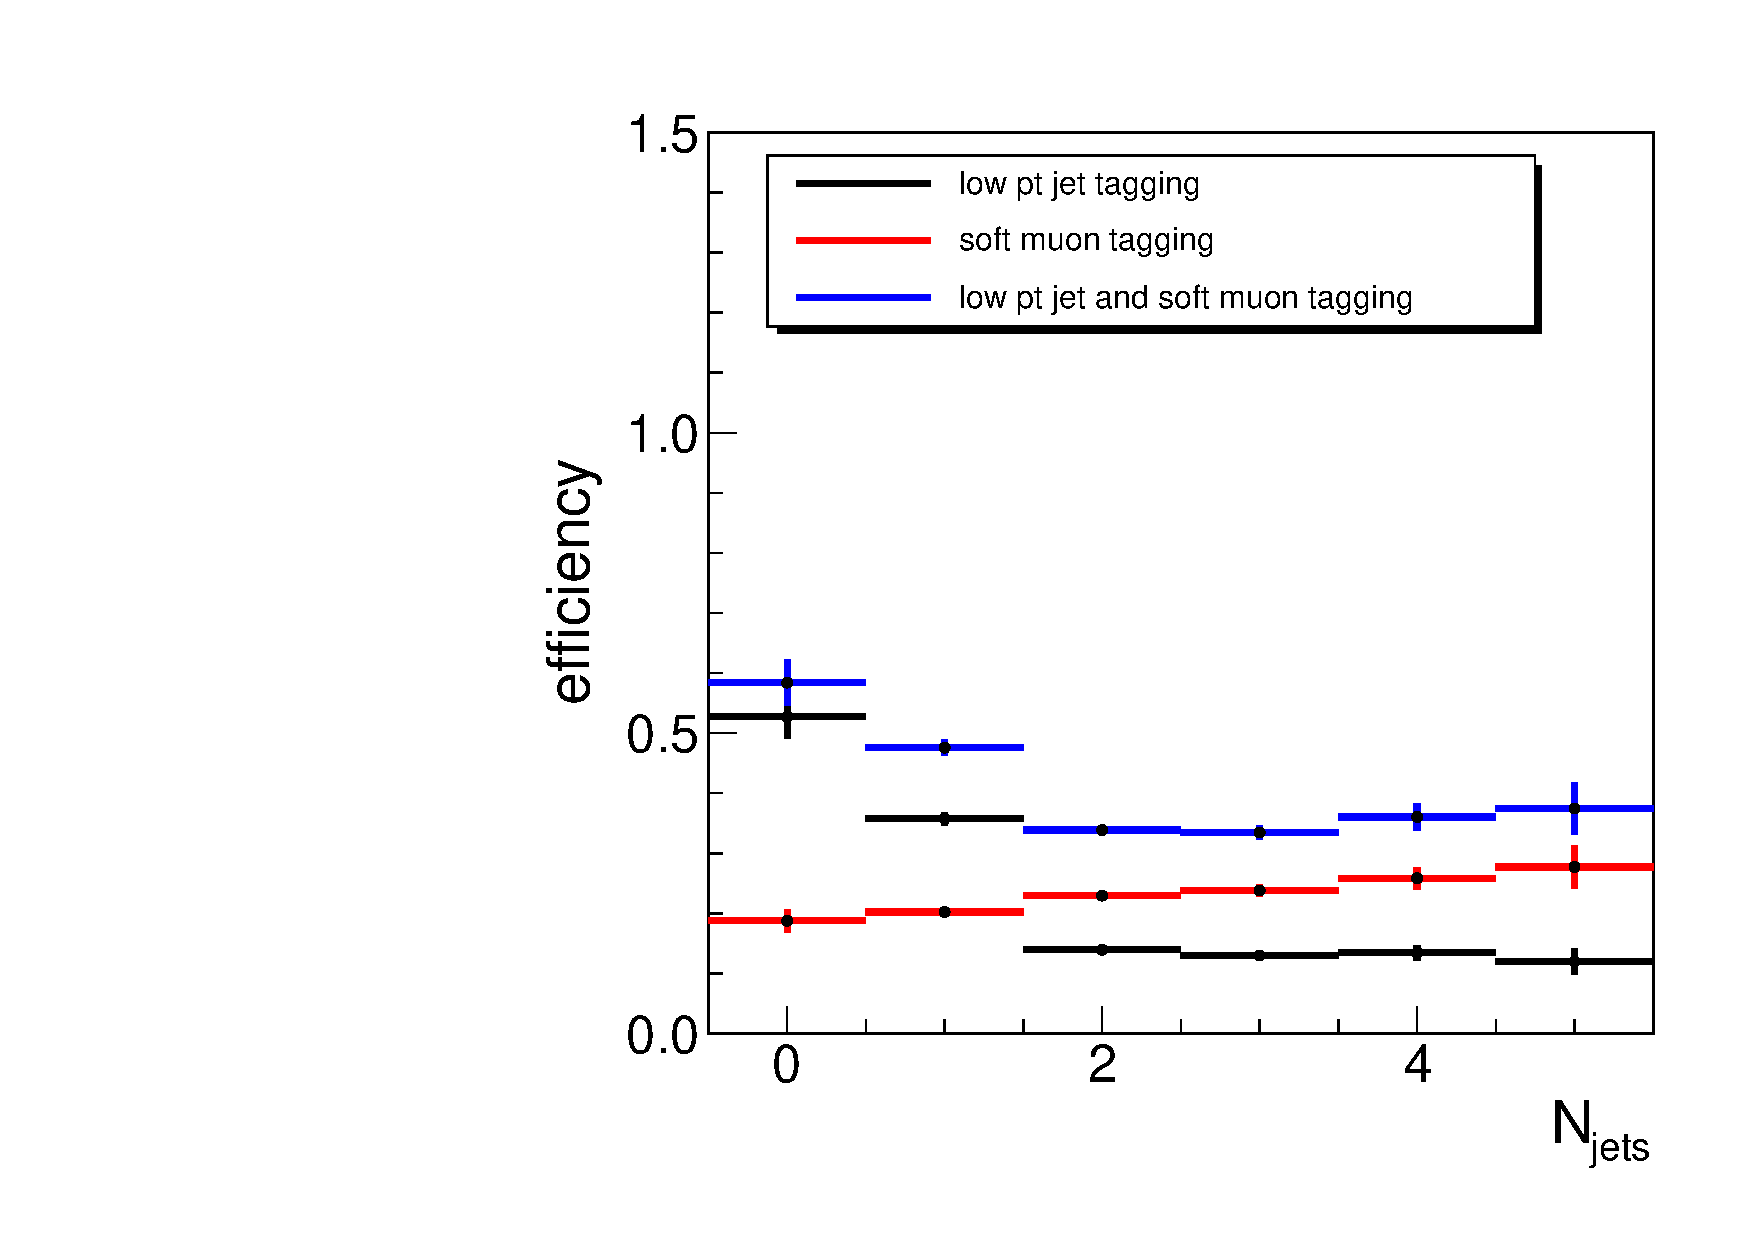
\includegraphics[width=0.55\textwidth]{figures/btag_njets_lowpttagging.pdf}
\caption{Tagging efficiency for low $\pt$ jets, soft muon tagging efficiency 
and the combination of both of them as a function of the number of reconstructed 
jets in top events after applying the $\WW$-like selection.}
\label{fig:btag_njets_lowpttagging}
\end{center}
\end{figure}

%
% ONE JET BIN
%
\subsubsection{1-Jet Bin Method}
To measure the tagging efficiency in the 1-jet bin we use top events 
with two reconstructed jets as a control sample. 
The expected tagging efficiency in simulated $t\bar{t}$ events after the $WW$ preselection
is shown using all jets and soft-muons and for the highest $\pt$ jet only
as a function of the number of counted jets in Figure~\ref{fig:btag_njets_highestptjet}.
%The total tagging efficiency might be expected to depend on the the jet bin because
%of differing jet kinematics.
%Even so, 
The tagging efficiency for the highest $\pt$ jet is approximately
the same for the 1-jet and 2-jet bins.
%, and does not depend on the topology of
%the other jets, as seen in Figure~\ref{fig:btag_njets_highestptjet}. 
Therefore, we propose to use the tagging on the highest $\pt$ jet
and measure the tagging efficiency in
the 2-jet bin. 

\begin{figure}[!htbp]
\begin{center}
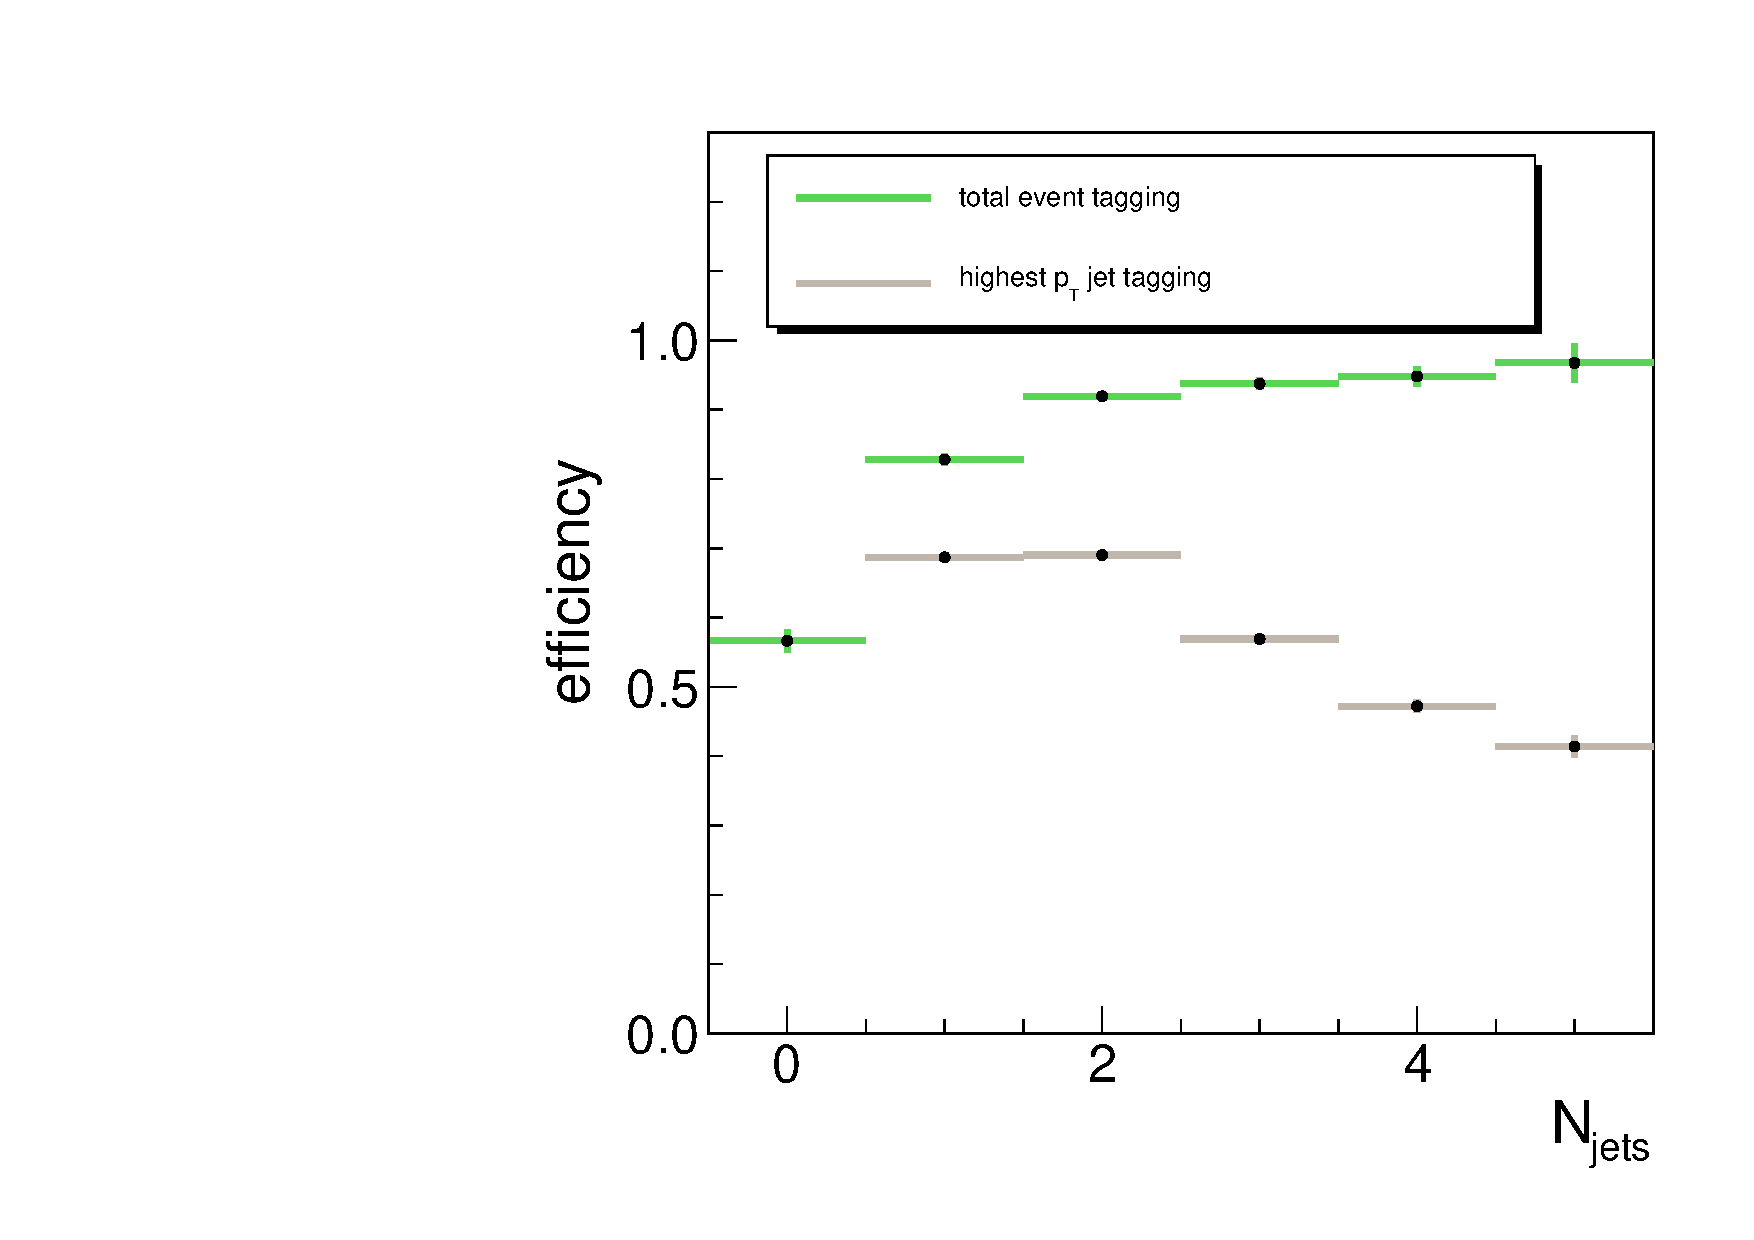
\includegraphics[width=0.55\textwidth]{figures/btag_njets_highestptjet.pdf}
\caption{Total tagging efficiency and tagging efficiency for the highest
$\pt$ jet as a function of the number of reconstructed
jets in top events after applying the $\WW$-like selection.}
\label{fig:btag_njets_highestptjet}
\end{center}
\end{figure}

The residual number of top events in the 1-jet bin is then given by,
$${N_{no~tagged}^{1-jet} = N_{tagged}^{1-jet} \times (1-\epsilon_{highest~\pt~jet})/\epsilon_{highest~\pt~jet}},$$
where $N_{tagged}^{1-jet}$ is the number of tagged events and $\epsilon_{highest~\pt~jet}$ is the tagging efficiency.
The closure test with simulated events agrees 
well within the statistical uncertainty.

%
% VBF! VBF! VBF!
% 
\subsubsection{2-Jet Bin Method}
Estimation of the top background in the 2-jet bin is complicated
by the additional kinematic requirements applied to the jets to
select qqH-like events.
The total tagging efficiency for the highest $\pt$ jet as a function
of the number of counted jets in simulated
$t\bar{t}$ events after requiring $\Delta \eta_{j1j2}>4$,
$m_{j1j2}>500~\GeVcc$ and $\eta_{j1}\eta_{j2}<0$ is shown in 
Figure~\ref{fig:btag_njets_vbfcuts}.
Although the number of simulated events meeting these requirements
is small, a trend towards lower efficiency in the 2-jet bin is observed
when compared with the behavior in Figure~\ref{fig:btag_njets_highestptjet}.
This is consistent with the expectation for this kinematic selection.

\begin{figure}[!htbp]
\begin{center}
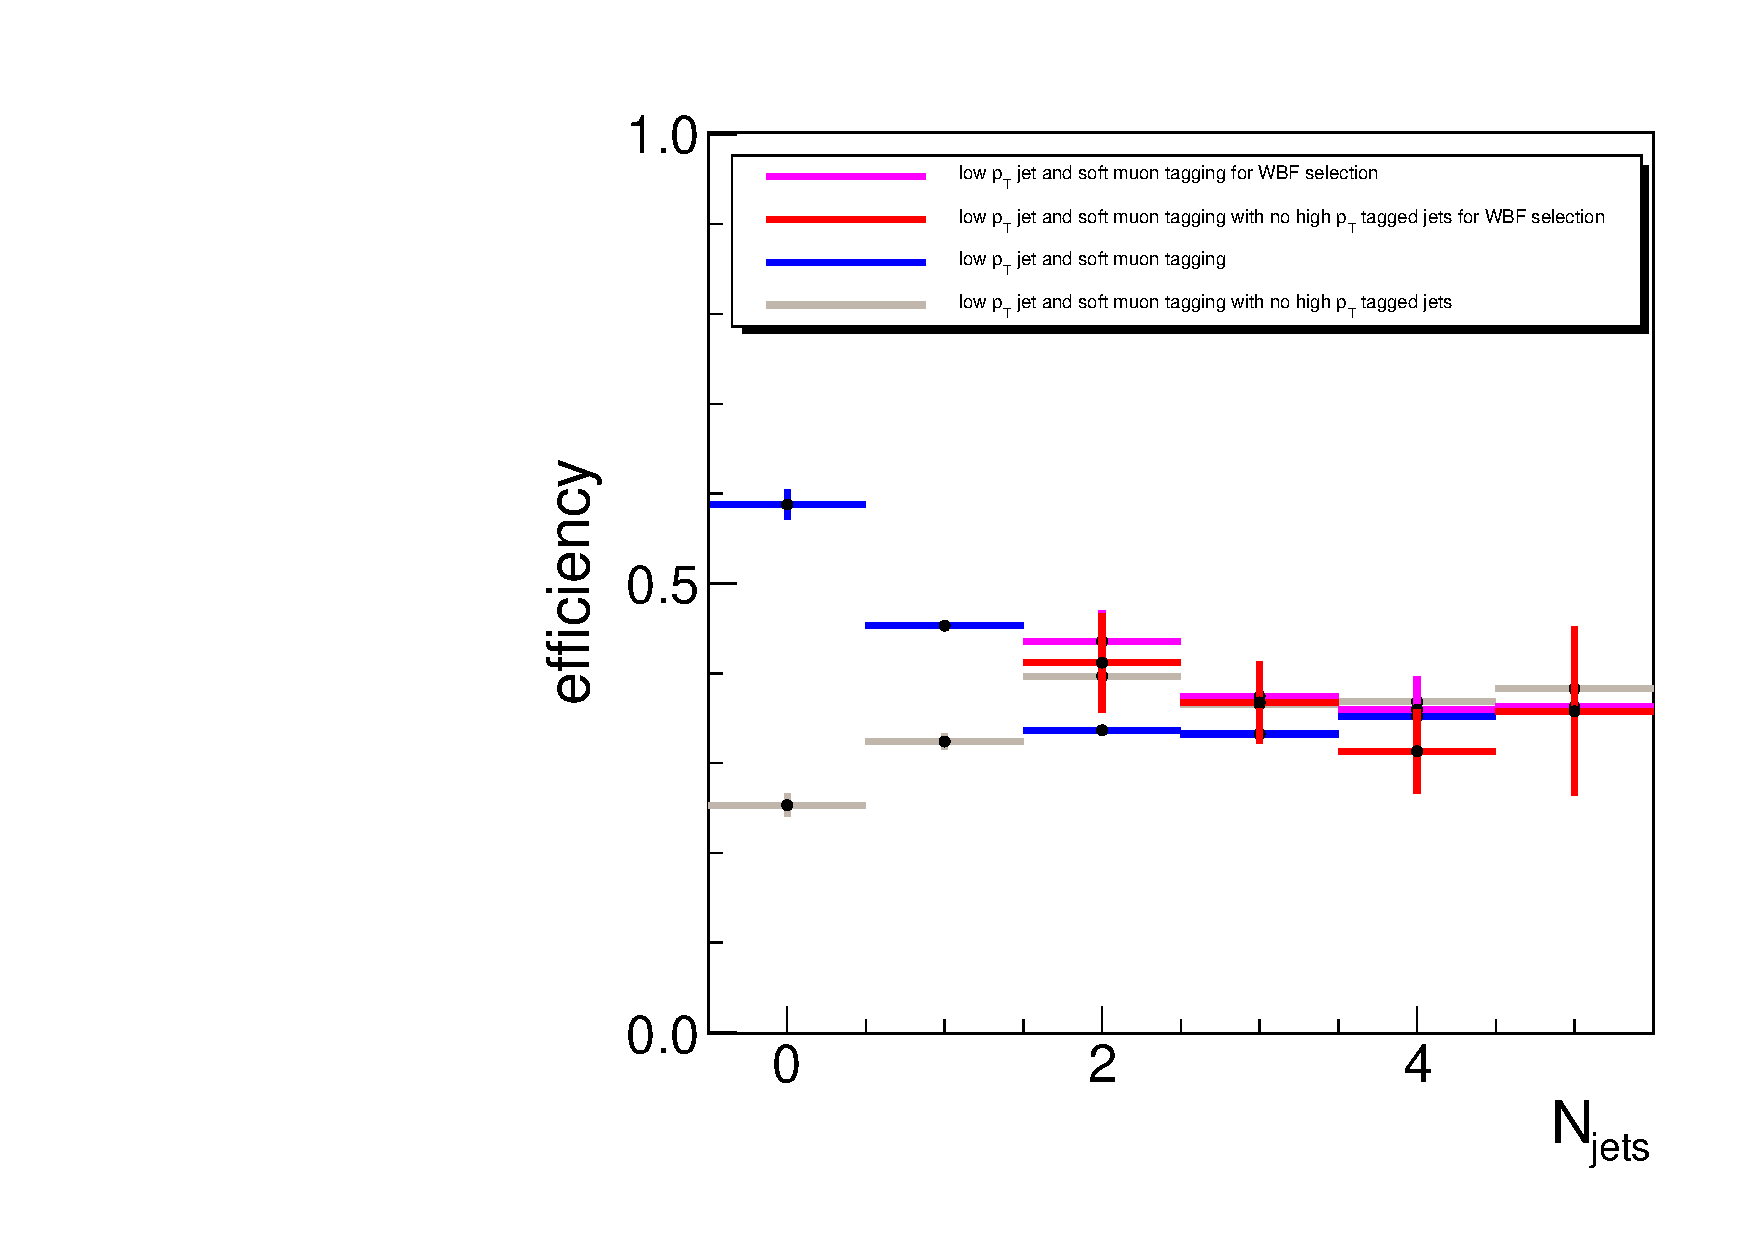
\includegraphics[width=0.55\textwidth]{figures/btag_njets_vbfcuts.pdf}
\caption{Total tagging efficiency and tagging efficiency for the highest 
$\pt$ jet as a function of the number of counted 
jets in top events after applying the $\WW$-like selection and a qqH-like selection.}
\label{fig:btag_njets_vbfcuts}
\end{center}
\end{figure}

The proposed method is to extract the tagging efficiency for the leading and 
trailing jet as a function of jet $\eta$ and $\pt$. 
This efficiency is then applied to untagged simulated top events. 
The tagging efficiency for low $\pt$ jets and soft muons is also measured from data.

%
% ON DATA
%
\subsubsection{Results}
This section describes the tagging efficiency results obtained in data, 
and the comparison of the residual background predictions obtained from
the methods described above with simulation expectations.

The tagging efficiency for the combination of low $\pt$ jets 
and soft muons as a function of the number of counted jets on data and 
simulation is shown in Figure~\ref{fig:btag_njets_lowpttagging_data}. 
The total tagging efficiency as a function of the number of reconstructed jets on data 
and simulation is shown in Figure~\ref{fig:btag_njets_totaltagging_data}. 
The tagging efficiency for the leading jet $\pt$ as a function of the number of 
reconstructed jets on data and simulation is shown in 
Figure~\ref{fig:btag_njets_highestptjet_data}. 
In all cases a reasonable agreement is found between the data 
and the simulation, although the statistical uncertainty is large.

\begin{figure}[!htbp]
\begin{center}
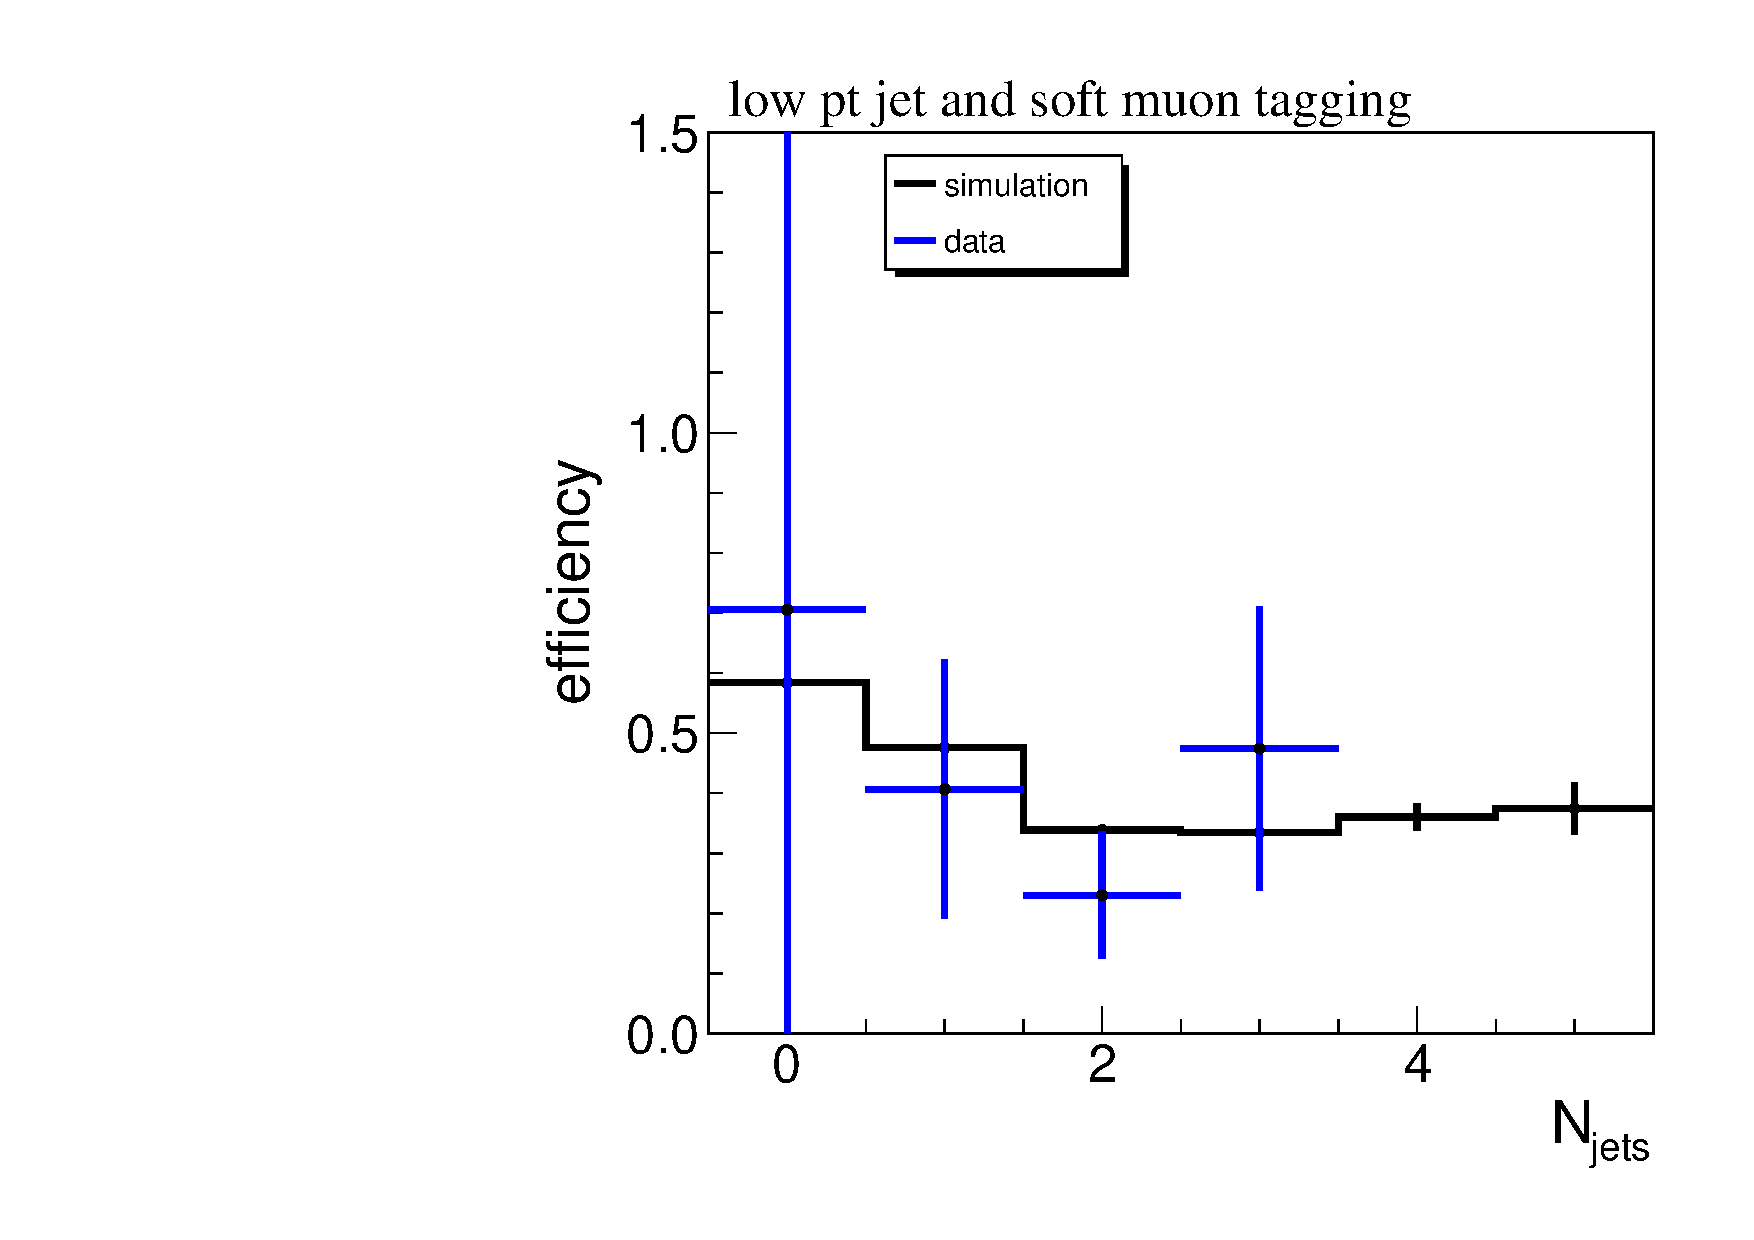
\includegraphics[width=0.55\textwidth]{figures/btag_njets_lowpttagging_data.pdf}
\caption{Tagging efficiency for the combination of low $\pt$ jets and soft muons 
as a function of the number of counted jets after applying 
the $\WW$-like selection on data and simulation.}
\label{fig:btag_njets_lowpttagging_data}
\end{center}
\end{figure}

\begin{figure}[!htbp]
\begin{center}
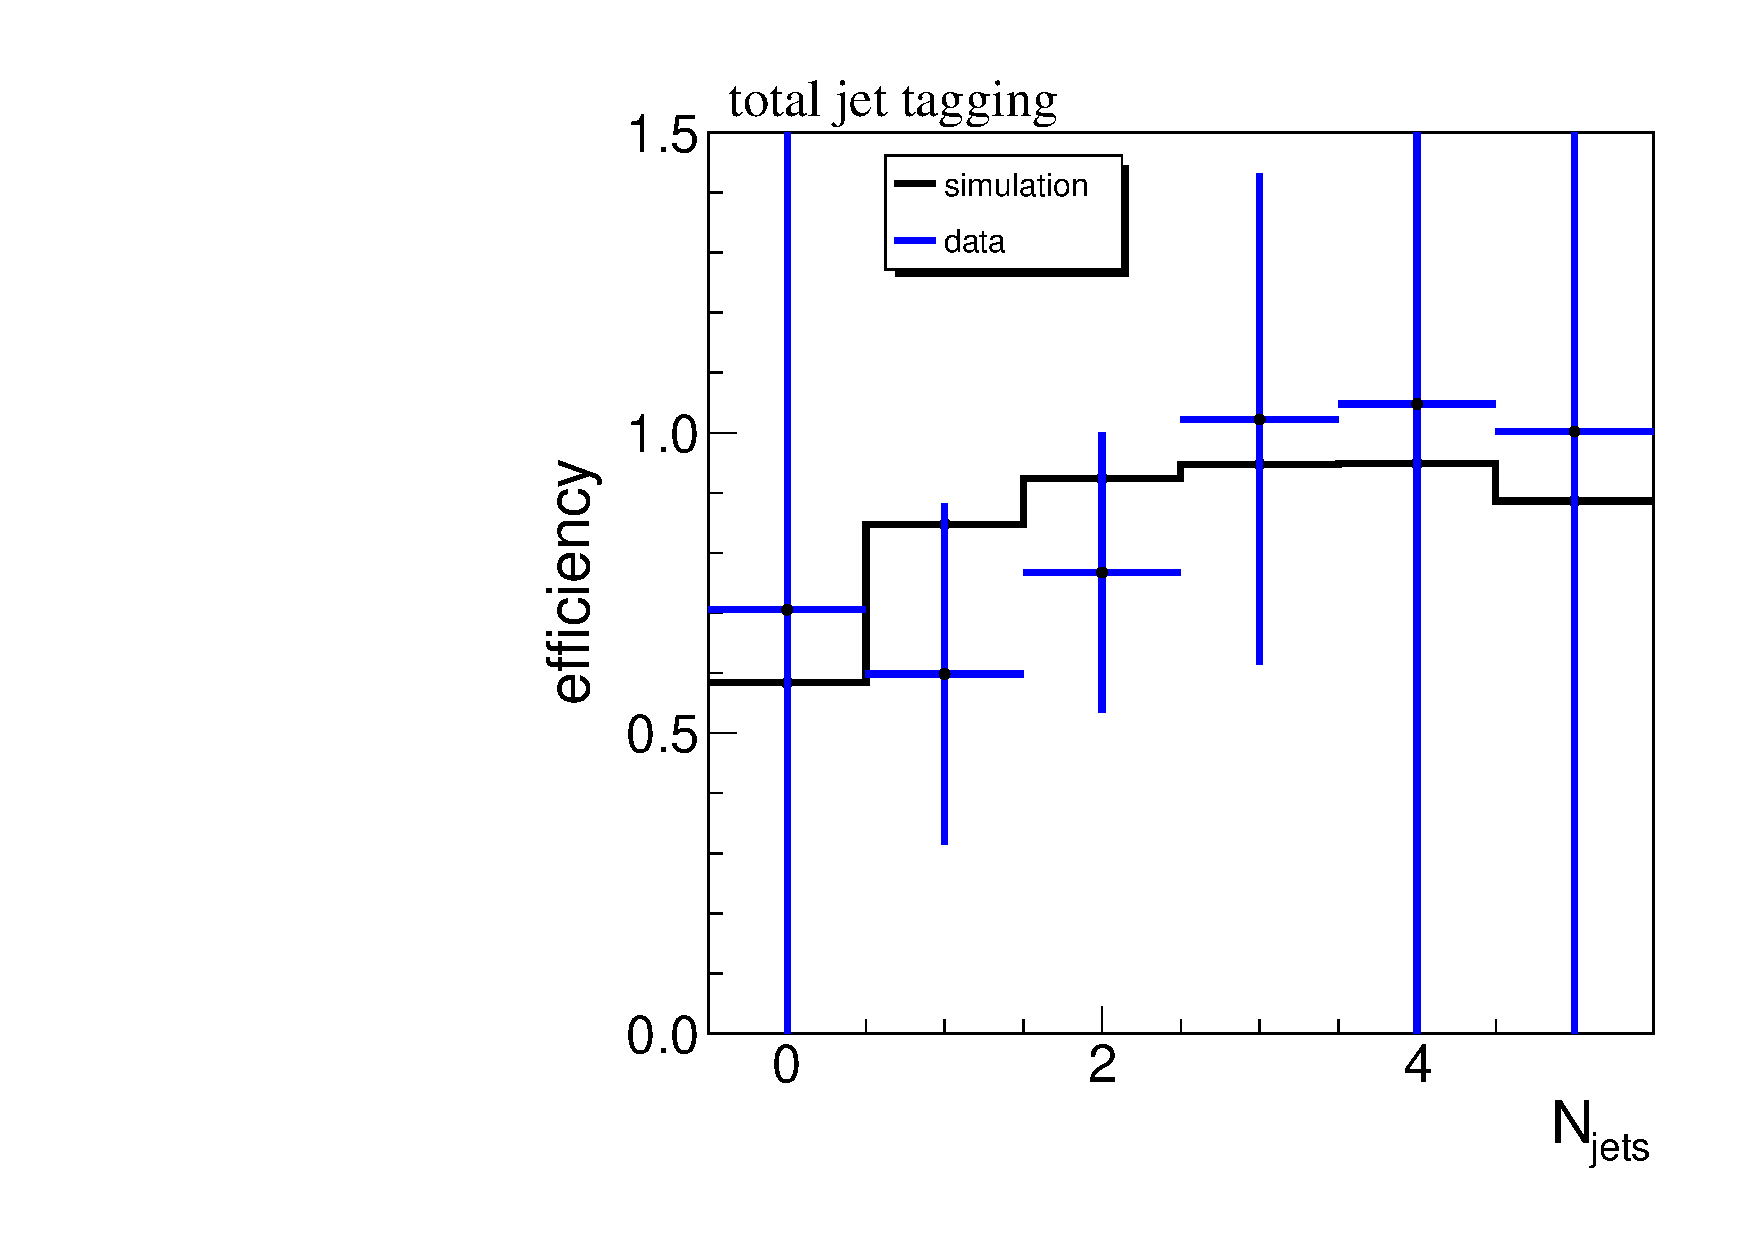
\includegraphics[width=0.55\textwidth]{figures/btag_njets_totaltagging_data.pdf}
\caption{The total tagging efficiency as a function of the number of counted 
jets after applying the $\WW$-like selection on data and simulation.}
\label{fig:btag_njets_totaltagging_data}
\end{center}
\end{figure}

\begin{figure}[!htbp]
\begin{center}
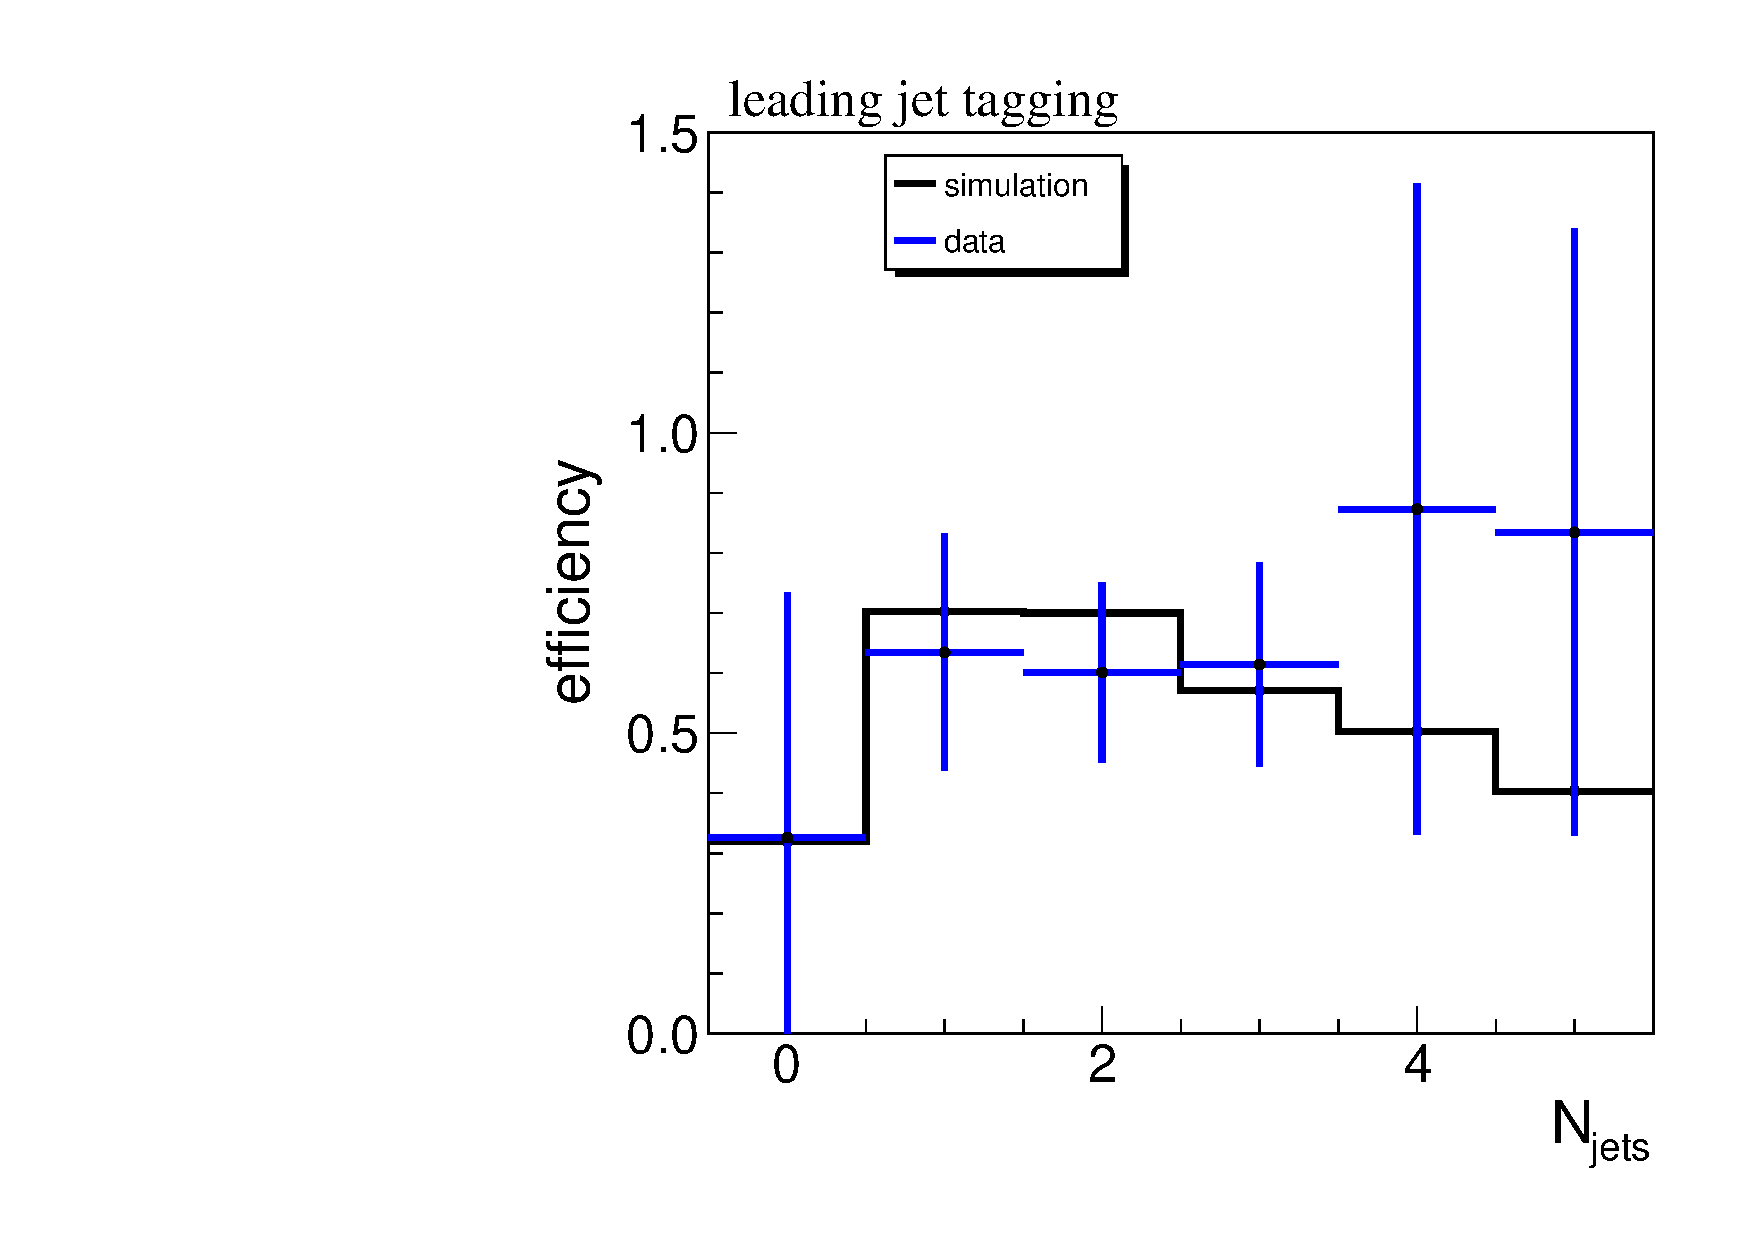
\includegraphics[width=0.55\textwidth]{figures/btag_njets_highestptjet_data.pdf}
\caption{Tagging efficiency for the leading jet $\pt$ as a function of the number of counted 
jets after applying the $\WW$-like selection on data and simulation.}
\label{fig:btag_njets_highestptjet_data}
\end{center}
\end{figure}

